\documentclass[11pt]{article}

\usepackage[utf8]{inputenc}
\usepackage[T1]{fontenc}
\usepackage{amsmath}
\usepackage{amssymb}
\usepackage{mathtools}
\usepackage{graphicx}
\usepackage{float}
\usepackage[left=10mm,right=10mm]{geometry}
\usepackage{booktabs}
\usepackage{array}
\usepackage{enumitem}
\usepackage{fancyhdr}
\usepackage{subfig}
\usepackage[ruled, lined, vlined, linesnumbered, commentsnumbered, longend]{algorithm2e}
\usepackage[activate={true,nocompatibility},final,tracking=true,kerning=true,spacing=true,factor=1100,stretch=10,shrink=10]{microtype}
\usepackage[margin=10pt,font=small,labelfont=bf,labelsep=endash]{caption}

% Refererencing
\usepackage[backend=biber,style=alphabetic]{biblatex}

\microtypecontext{spacing=nonfrench}

\graphicspath{ {./images/} }

\newcolumntype{L}[1]{>{\raggedright\arraybackslash}p{#1}}

\newcommand{\derivative}[2]{\frac{\partial #1}{\partial #2}}
\newcommand{\suml}[2]{\sum\limits_{#1}^{#2}}

\pagestyle{fancy}
\fancyhf{}
\setlength{\headheight}{14pt}
\rhead{\thepage}
\lhead{Assignment 4}

\begin{document}
\title{\textbf{\huge{Title}}}

\date{\today}
\author{Sanchit Nevgi}

\section{Derivation of conditional distribution}
The probability distribution over a vector $y \in \{-1,+1\}^d$ is given by,

\[ p(y \vert b,w) = \frac{1}{Z} \prod_{i=1}^d \exp( b_i y_i ) \prod_{(i,j)\in \text{pairs}} \exp(w_{ij} y_i y_j). \]

By conditional probability $p(a, b) = p(a | b) p(b)$
\begin{equation}
    \begin{aligned}
        p(y | b, w) &= p(y_i | y_{-i}, b, w) p(y_{-i} | b, w) \\
        p(y_i | y_{-i}, b, w) &=  \frac{p(y | b, w)}{p(y_{-i} | b, w)} \\
        &= \frac{p(y | b, w)}{\sum\limits_{y_i} p(y | b, w)} \\
        p(y_i = 1, y_{-i} | b, w) &= \frac{p(y | b, w)}{p(y_{-i}, y_i=-1 | b, w) + p(y_{-i} | y_i = 1, b, w)} \\
        & \medskip \;\;\;\; \textit{Substituting the probability definition} \\
        &= \frac{1}{Z(y_{-i})} \frac{\prod_{k=1}^d \exp( b_k y_k ) \prod_{(k,j)\in \text{pairs}} \exp(w_{kj} y_k y_j)}{\sum_{y_k} \prod_{k=1}^d \exp( b_k y_k ) \prod_{(k,j)\in \text{pairs}} \exp(w_{kj} y_k y_j)}
    \end{aligned}
\end{equation}

The common terms in the numerator and denominator cancel out, and only the terms that contain $i$ survive. Further we substitute both values of $y_i$. Note, that the normalizing constant depend on $y_{-i}$

\begin{equation}
    \begin{aligned}
        p(y_i = 1 | y_{-i}, b, w) &= \frac{\exp (b_i) \prod_{j \in nb(i)} \exp (w_{ij} y_j)}{\exp (-b_i) \prod_{j \in nb(i)} \exp (-w_{ij} y_j) +  \exp (b_i) \prod_{j \in nb(i)} \exp (w_{ij} y_j)} \\
        & \medskip \;\;\;\; \textit{Since, } \exp(a) \exp(b) = \exp(a + b) \\
        &= \frac{\exp(b_i + \sum_{j \in nb(i)} w_{ij} y_j)}{\exp(-b_i - \sum_{j \in nb(i)} w_{ij} y_j) + \exp(b_i + \sum_{j \in nb(i)} w_{ij} y_j)} \\
        & \medskip \;\;\;\; \textit{Dividing by the numerator} \\
        &= \frac{1}{1 + \exp(- 2(b_i + \sum_{j \in nb(i)} w_{ij} y_j)))} \\
        &= \sigma(2(b_i + \sum_{j \in nb(i)} w_{ij} y_j)) \;\;\;\; \text{Since,} \;\; \sigma(x) = 1 / (1 + \exp(-x))
    \end{aligned}
\end{equation}

\section{Pseudo-Code for Gibbs Sampling}

\begin{algorithm}[H]
    \SetAlgoLined
    \tcc{Input model parameters and number of iterations}
    \KwIn{$t_{max}$, b, w}
    Init $y^0 \in \mathbb{R}^d$ \;
    \For {$t \gets 1$ to $t_{max}$}{
    $y^t \gets y^{t-1}$ \;
    \tcc{Iterate over the dimensions}
      \For {$i \gets 1$ to $d$}{
        \tcc{Sample $r \in \{ -1, 1 \}$ from the conditional distribution}
        $r \backsim P(Y_i | Y_{-i} = y_{-i}^t, b, w)$ \;
        $y_i^t \gets r$
      } 
     }
     \Return{$y^0$, ..., $y^{t_{max}}$}
     \caption{Gibbs Sampling}
\end{algorithm}

\section{Samples}

\begin{figure}[H]%
    \centering
    \subfloat[]{{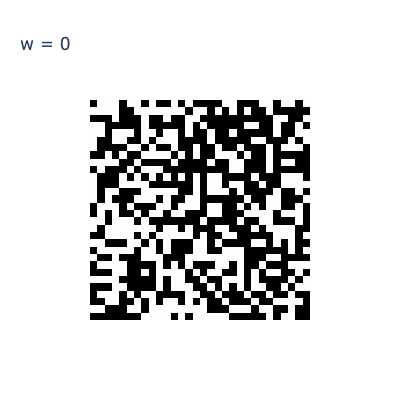
\includegraphics[width=5cm]{./images/sample-1.png} }}%
    \subfloat[]{{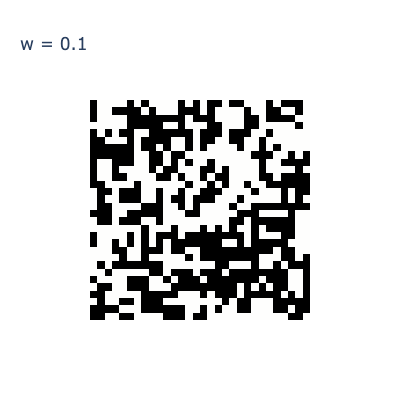
\includegraphics[width=5cm]{./images/sample-2.png} }}%
    \subfloat[]{{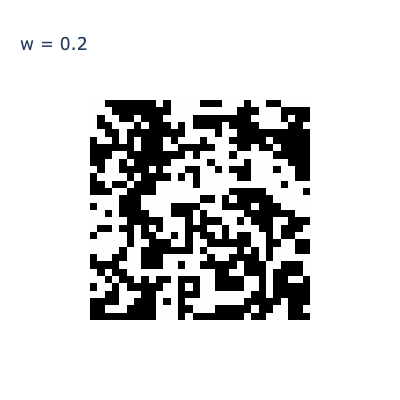
\includegraphics[width=5cm]{./images/sample-3.png} }}%
    \qquad
    \subfloat[]{{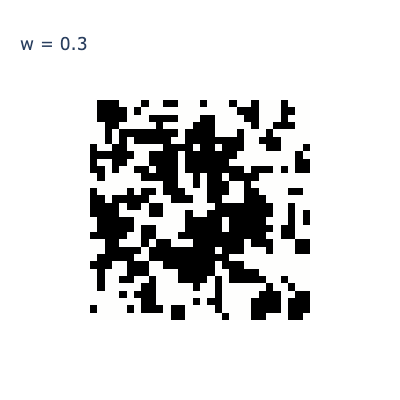
\includegraphics[width=5cm]{./images/sample-4.png} }}%
    \subfloat[]{{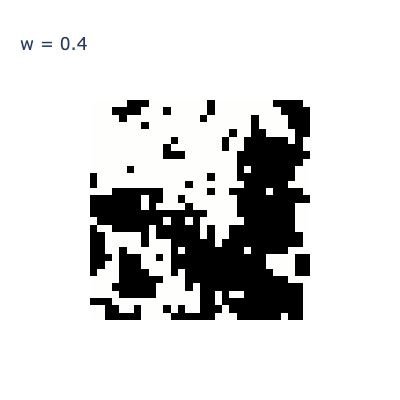
\includegraphics[width=5cm]{./images/sample-5.png} }}%
    \subfloat[]{{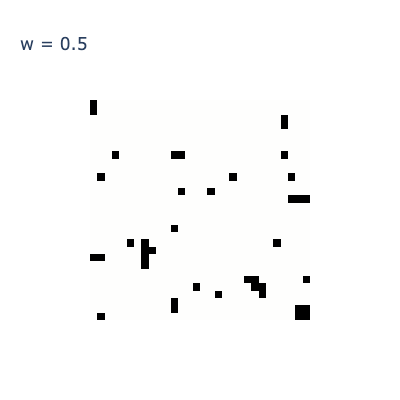
\includegraphics[width=5cm]{./images/sample-6.png} }}%
    \qquad
    \caption{Samples obtained from Gibbs algorithm over 100 iterations for $\tilde{w} \in \{0. .1, .2, .3, .4, .5\}$. $y$ initialzed as $\{+1\} \in \mathbb{R}^d$}%
\end{figure}

\section{Discussion}

Given the probability distribution $(y | b, w) \propto \exp(w_{i,j} y_i, y_j)$, we see that for higher values of $w_{ij}$, the neighbouring pixels are inclined to have the same value. Initially, the images are $\{+1\}^d$ and progressively they form larger regions of pixels with the same values. For large values of w $\ge 0.5$, the images are mostly white, due to the initialization.

\section{Mixing Times}

\begin{figure}[H]%
    \centering
    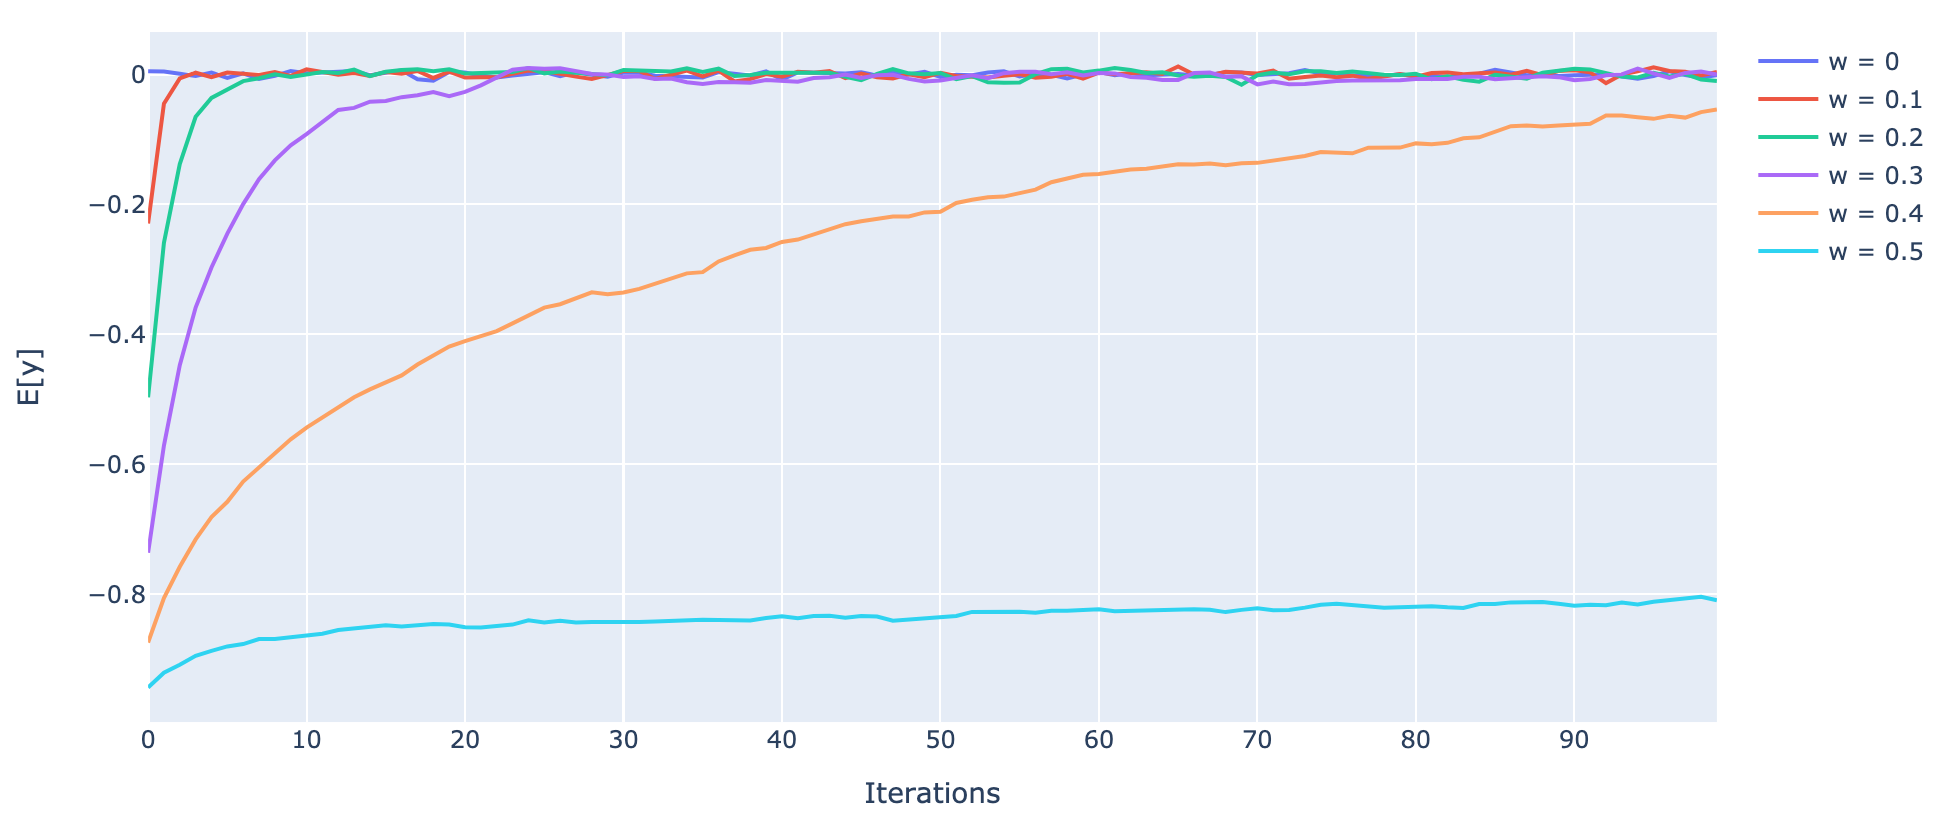
\includegraphics[width=0.8\textwidth]{./images/normalized-labeled.png}
    \caption{Plot of the E[y] over 100 independent Markov chains for $\tilde{w} \in \{0. .1, .2, .3, .4, .5\}$, when initialized with $\{-1\}^d$}
\end{figure}

\section{Discussion}

We see that the rate of convergence of $E[y]$ is inversely proportional to the value of w; smaller $w \in \{ 0, .1, .2, .3, .4 \}$ converge to 0 within 100 iterations, while $w \in \{ 0.4, 0.5 \}$ have not yet converged. The quality of samples improves with the number of iterations. Since Gibbs sampling is initialized with $\{-1\}^d$, higher values of $w$, would want neighbouring pixles to have same values (-1)

\section{Fixed Parameter Denoising}

\begin{figure}[H]
    \centering
    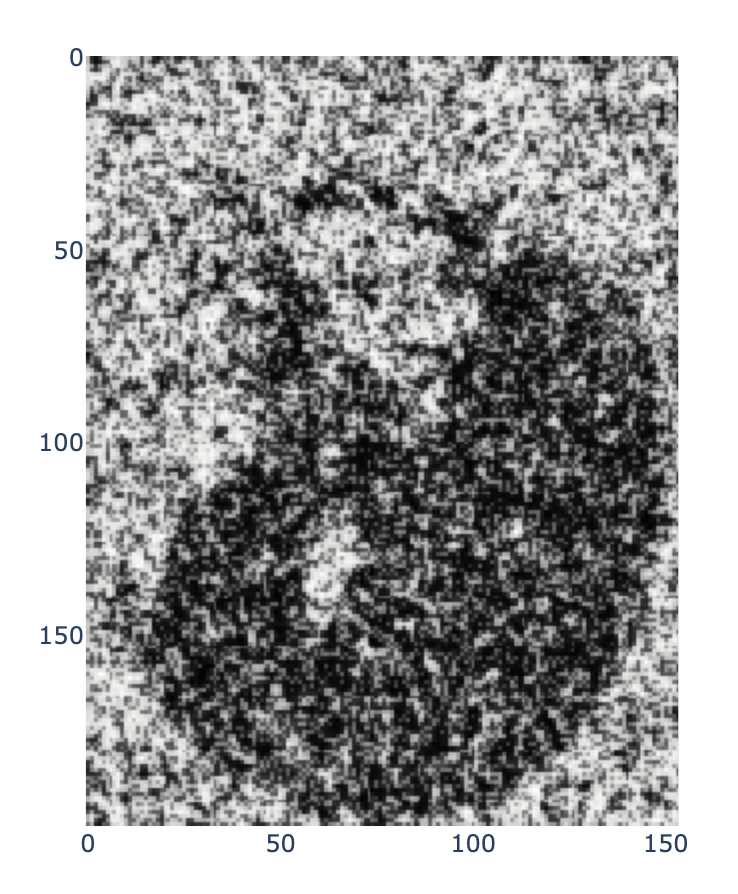
\includegraphics[width=0.4\textwidth]{./images/default-img-noisy.png}
    \caption{Mean image obtained from Gibbs with $w = 0.3$ and $b = 0.5$ }
\end{figure}

Per-pixel Averaged Mean Absolute Error = \texttt{0.65397}


\section{Varying Paramters}

The default values of $w_{ij} = 0.3$ and $b_i = 0.5$ give a $MAE = 0.65397$. From inital analysis, we see that for $\theta_2 > 10, \theta_1 > 2$, there is only a marginal improvement or degradation in MAE, as see in Figure. We limit the ranges of $\theta_1 \in [0, .5, 1, 2]$ and $\theta_2 \in [0, .3, 1, 5, 10]$.
We use a \textit{Grid Search} over this parameter space to find the best combination. We find that for $\theta_1 = 0.5$ and $\theta_2 = 5$, we get the lowest error. 

\noindent \textbf{Lowest Mean Absolute Error}: \texttt{0.1366}

\begin{figure}[H]
    \centering
    \subfloat[High $\theta_1$ value $\theta_1 = 2$, $MAE = 0.25$]{
        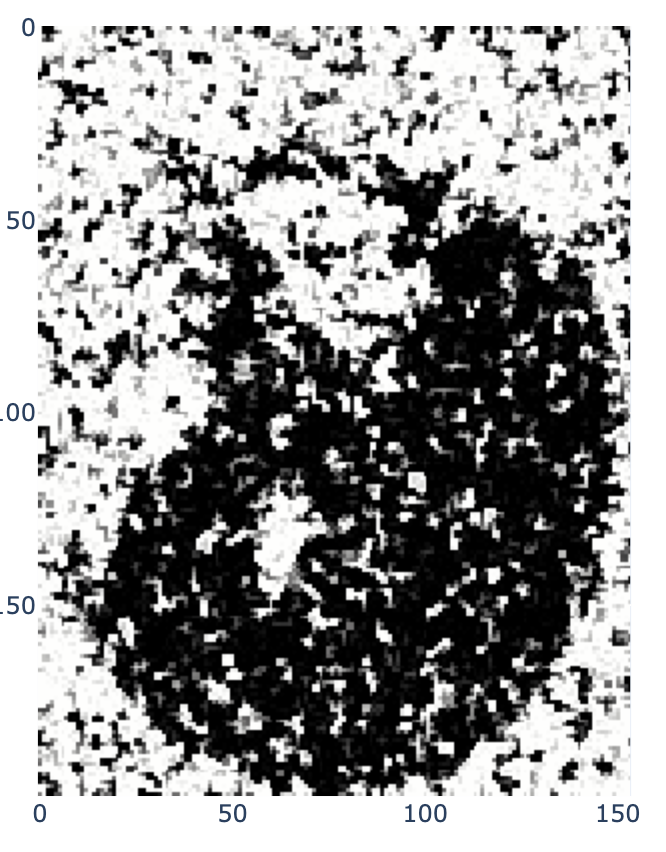
\includegraphics[width=0.32\textwidth]{./images/high-b.png}}%
    \subfloat[High $\theta_2$ value $\theta_2 = 10$, $MAE = 0.15$]{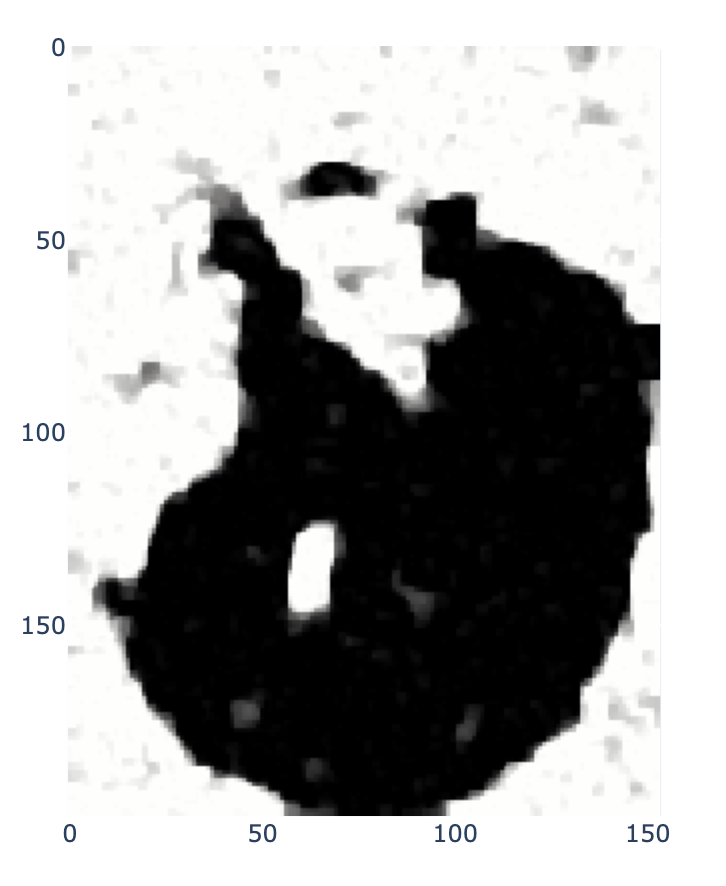
\includegraphics[width=0.32\textwidth]{./images/high-w.png}}
    \subfloat[Best image obtained from Gibbs with $\theta_2 = 5$ and $\theta_1 = 0.5$, $MAE = 0.136$]{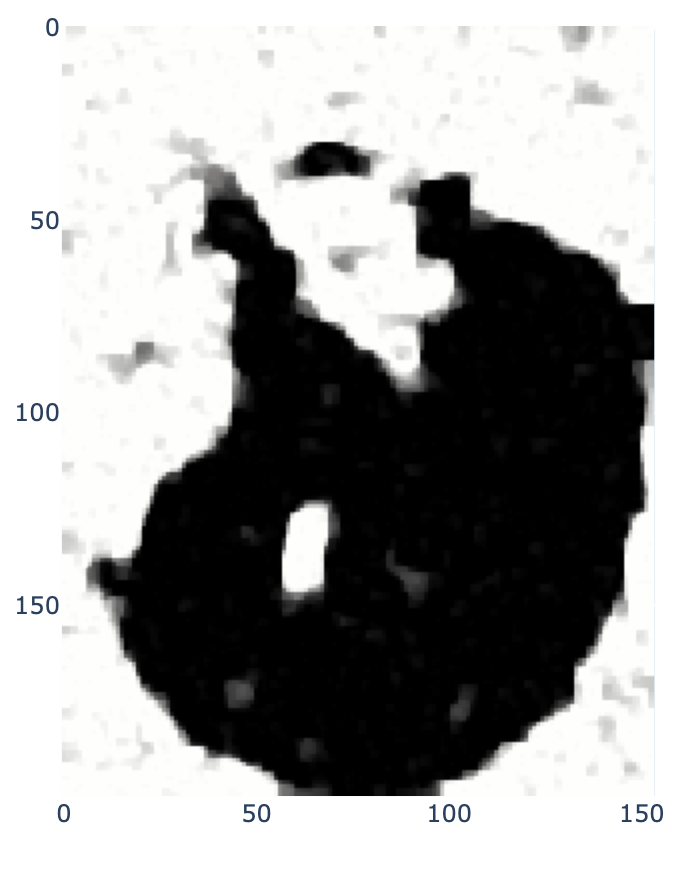
\includegraphics[width=0.32\textwidth]{./images/img-1.png}}
\end{figure}

\section{Varying w as a function of x}

We modify $w_{ij}$ such that it is dependent on $x$. Thus the new probability distribution $p(y|b, w) \propto \prod_{(i, j) \in pairs} \exp(\theta_2 f(x) y_i y_j)$. Having $f(x)$ term ensures that the samples obtained from the distribution "mimic" the noisy image. This could help preserving the \textit{details} from the noisy input.

For this experiment, we choose $f(x)$ as a convolution operation. $w_{i,j} = \sum_{k \in nb(x_{i,j})} f_k x_k$. The motivation behind this, is that using the neighbourhood of $x_{ij}$ would give a better estimate of the value of the $x_{i,j}$.

We define a \textit{Gaussian kernel} with filter sizes $f \in \{ 5, 7, 10, 20 \}$ and standard deviation $\sigma \in \{ 1, 2, 3 \}$. We perform a convolution operation on $x$ using this filter with appropriate padding. We take element-wise absolute value and the values bewtween $[3, 12]$ to obtain the final $w$. We see that a larger kernel size leads to more smoothing with a loss of detail.

\medskip \noindent \textbf{Mean Absolute Error} = \texttt{0.11} (+2\%) improvement

\begin{figure}[H]%
    \centering
    \subfloat[Best image, $MAE = 0.11$]{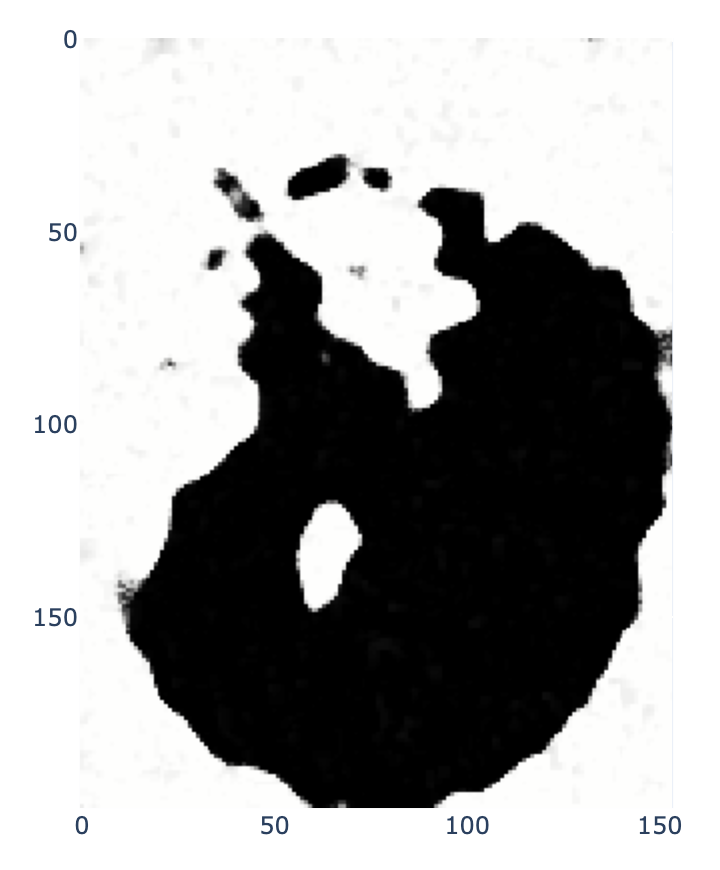
\includegraphics[width=0.32\textwidth]{./images/varying-x.png}}
    \subfloat[Gaussian Kernel]{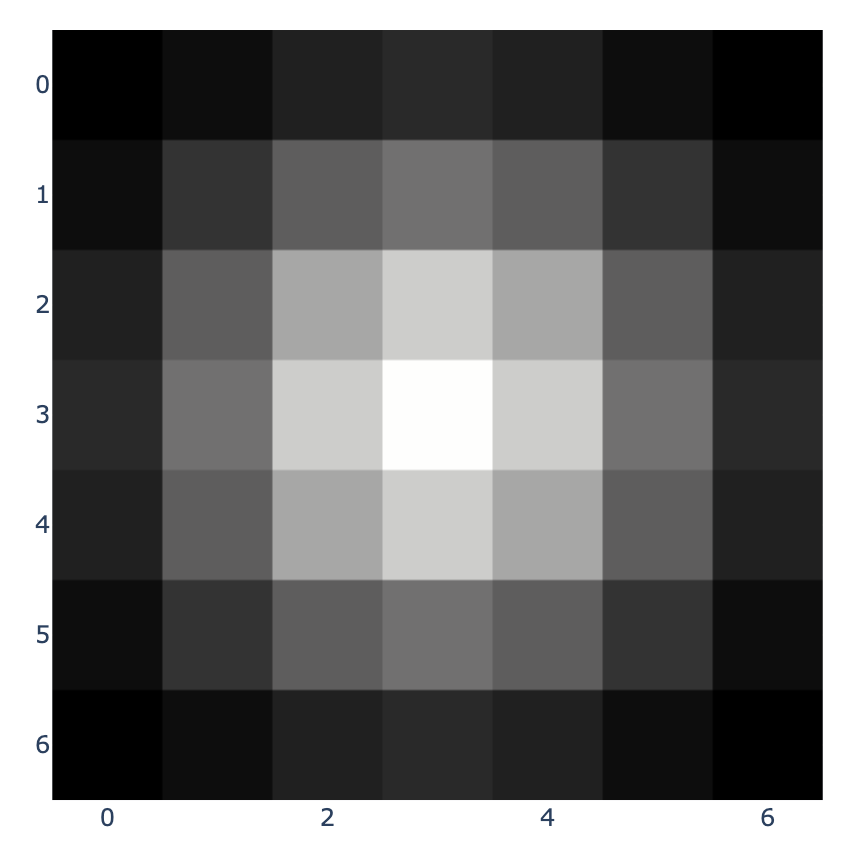
\includegraphics[width=0.32\textwidth]{./images/kernel.png}}
\end{figure}

\end{document}